\section{Beam Optics}

\todo{blabla}

% ============================================
%               Dispersion
% ============================================
\subsection{Dispersion}

Treating a beam as a single particle having the design momentum $p_0$ leads to a machine with no
apparent ill effect related to that momentum.
However, when considering a particle beam where each particle follows a distribution in
momentum, a few effects arise from this deviation, called the \textit{momentum offset},
$\delta$. It is defined as a relative difference to the design momentum:

\begin{equation}
    \delta = \frac{p - p_0}{p_0}.
    \label{eq:coordinate_systems:momentum_offset}
\end{equation}

Those effects are referred to as \textit{chromatic aberrations}. The first and most important to
consider is the \textit{dispersion}. Dispersion results from a particle with a momentum offset
being deflected differently by the dipoles compared to a particle at the design momentum.
Figure~\ref{fig:coordinate_systems:dispersion} shows an example of deflection. 

\begin{figure}[H]
    \centering
    \includegraphics[width=0.6\textwidth]{images/dipole.png}
    \caption{Particles with a momentum offset will be deflected differently by dipoles. This offset
            in position can be described by the dispersion function.}
    \label{fig:coordinate_systems:dispersion}
\end{figure}

The particle is still subject to the other properties of the lattice, but with a different orbit,
described by Eq.~\eqref{fig:coordinate_systems:dispersion}.

\begin{equation}
    \begin{aligned}
    D_x(s) = \frac{\Delta x(s)}{\delta} \\
    D_y(s) = \frac{\Delta y(s)}{\delta} \\
    \end{aligned}
    \label{eq:coordinate_systems:dispersion}
\end{equation}



% ============================================
%               Beta Beating
% ============================================
\subsection{\todo{$\beta$-beating}}


% ============================================
%                  Coupling
% ============================================
\subsection{\todo{Coupling}}


% ============================================
%         Momentum Compaction Factor
% ============================================
\subsection{\todo{Momentum Compaction Factor}}

